\section{Diagrama esquemático de la placa de expansión}
\label{sec:anexo_esquematico}

\begin{figure}[H]
    \centering
    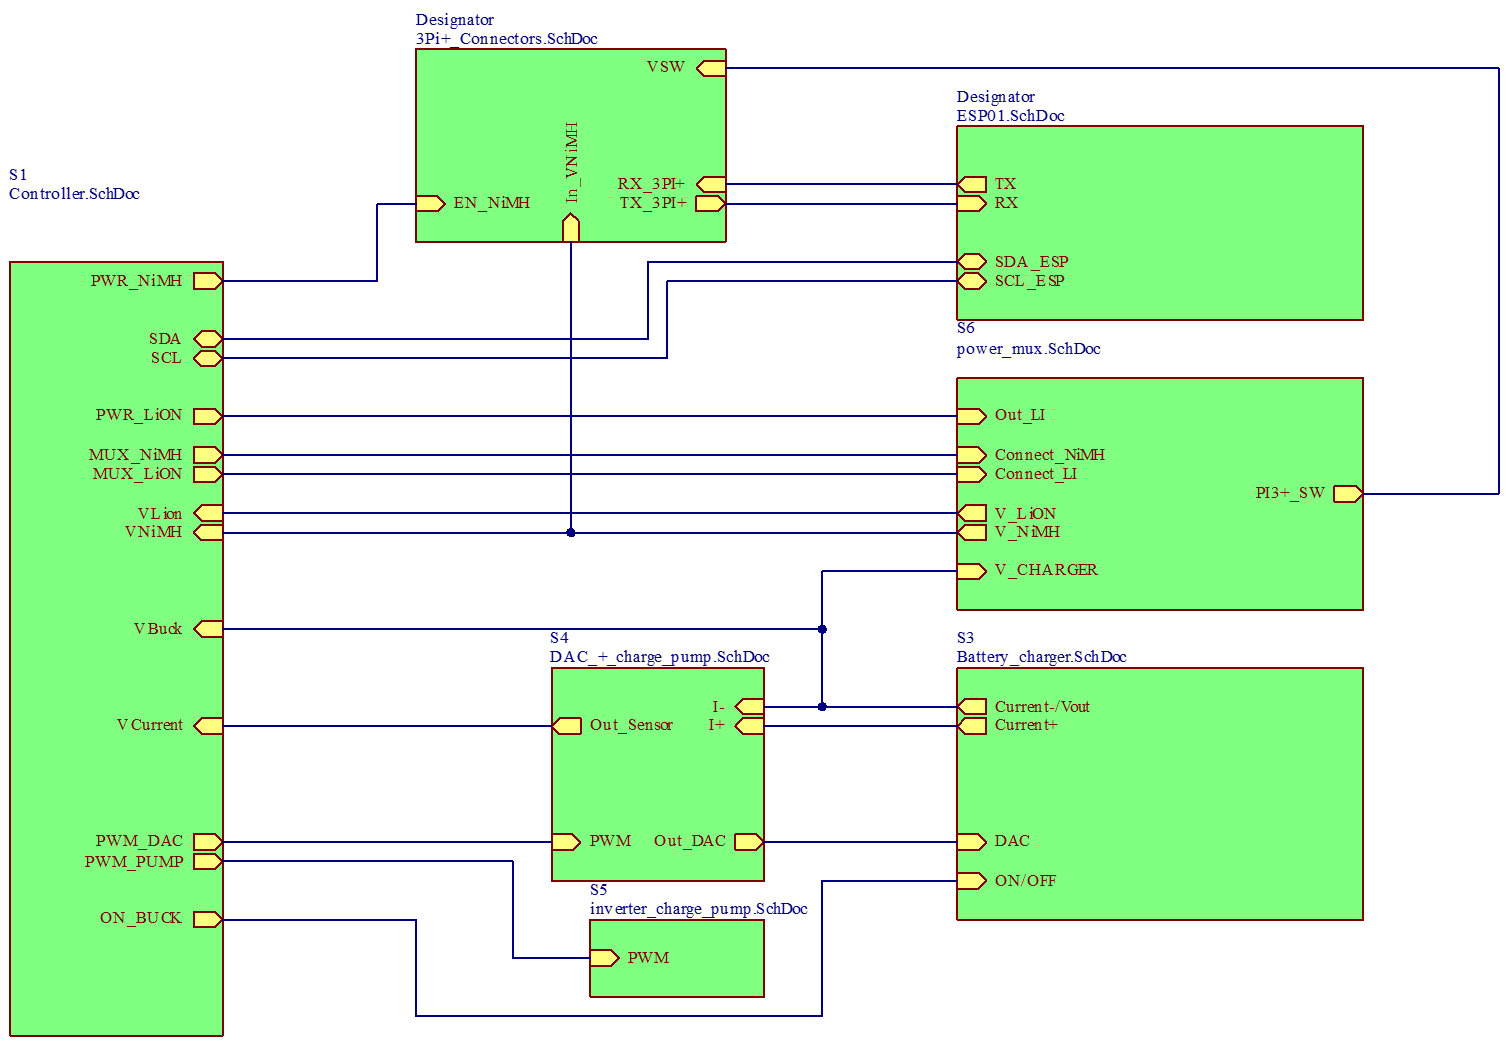
\includegraphics[scale=0.3]{imagenes/system_interconection.png}
    \caption{Interconexión de los circuitos en la placa de expansión}
    \label{fig:all}    
\end{figure}

\begin{figure}[H]
    \centering
    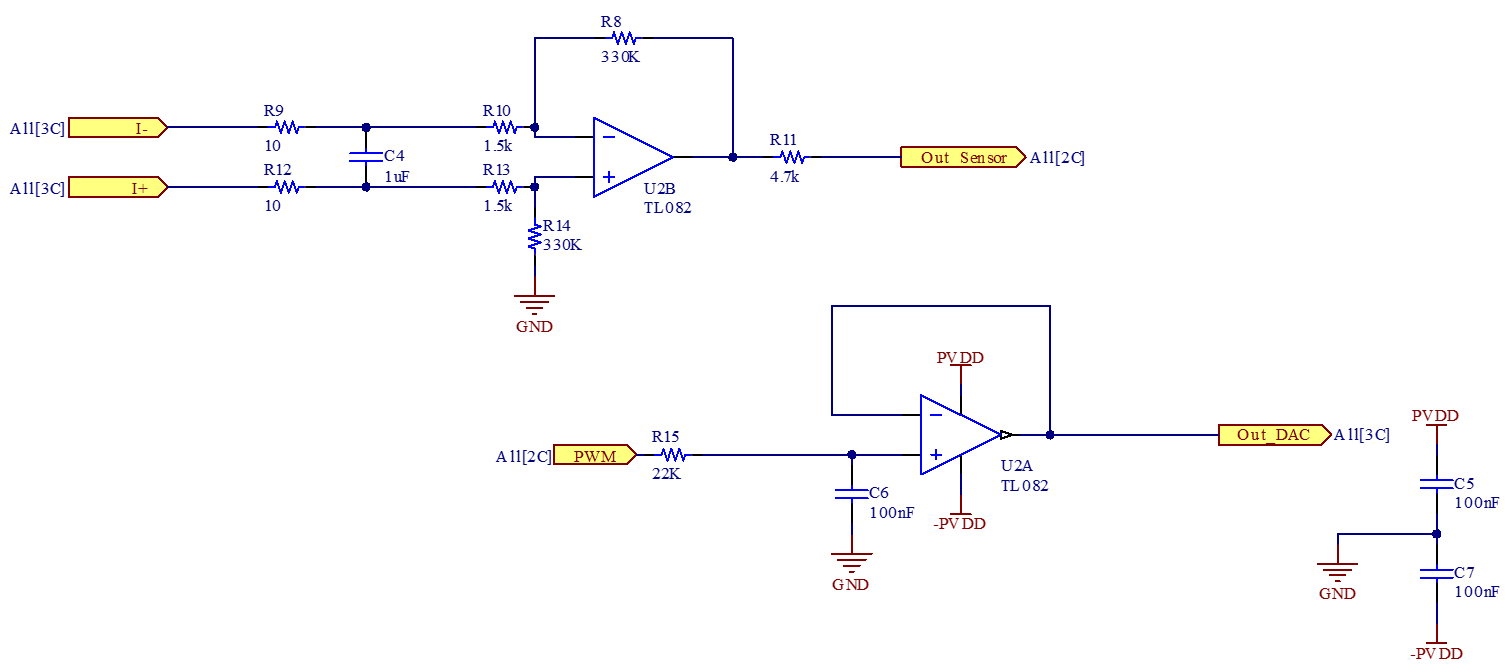
\includegraphics[scale=0.3]{imagenes/dac_sensor.png}
    \caption{Diagrama esquemático del sensor de corriente y el convertidor digital a analógico
    (S4 en la figura \ref{fig:all})}
    \label{fig:dac_sensor}
\end{figure}


\begin{figure}[H]
    \centering
    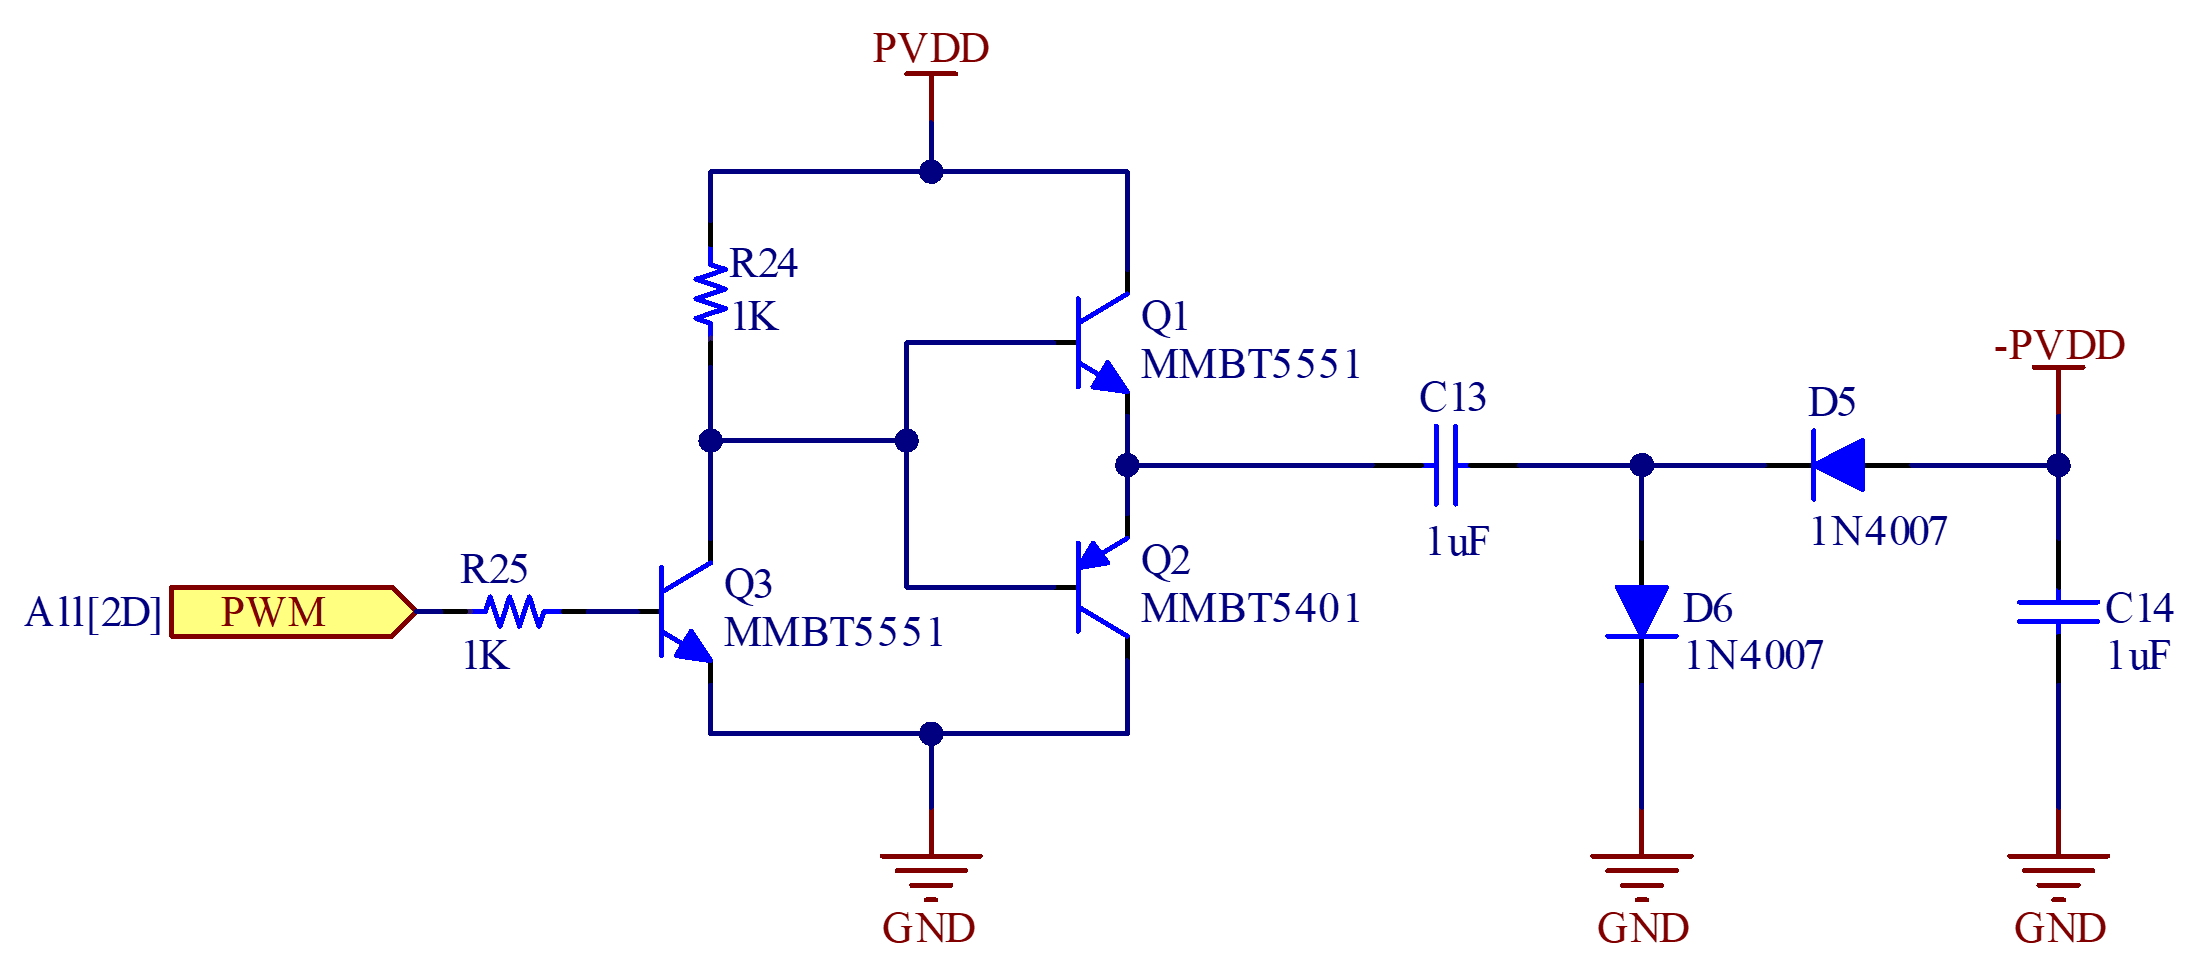
\includegraphics[scale=0.25]{imagenes/charge_pump.png}
    \caption{Diagrama esquemático del \textit{charge pump} (S5 en la figura \ref{fig:all})}
    \label{fig:charge_pump_anexo}
\end{figure}


\begin{figure}[H]
    \centering
    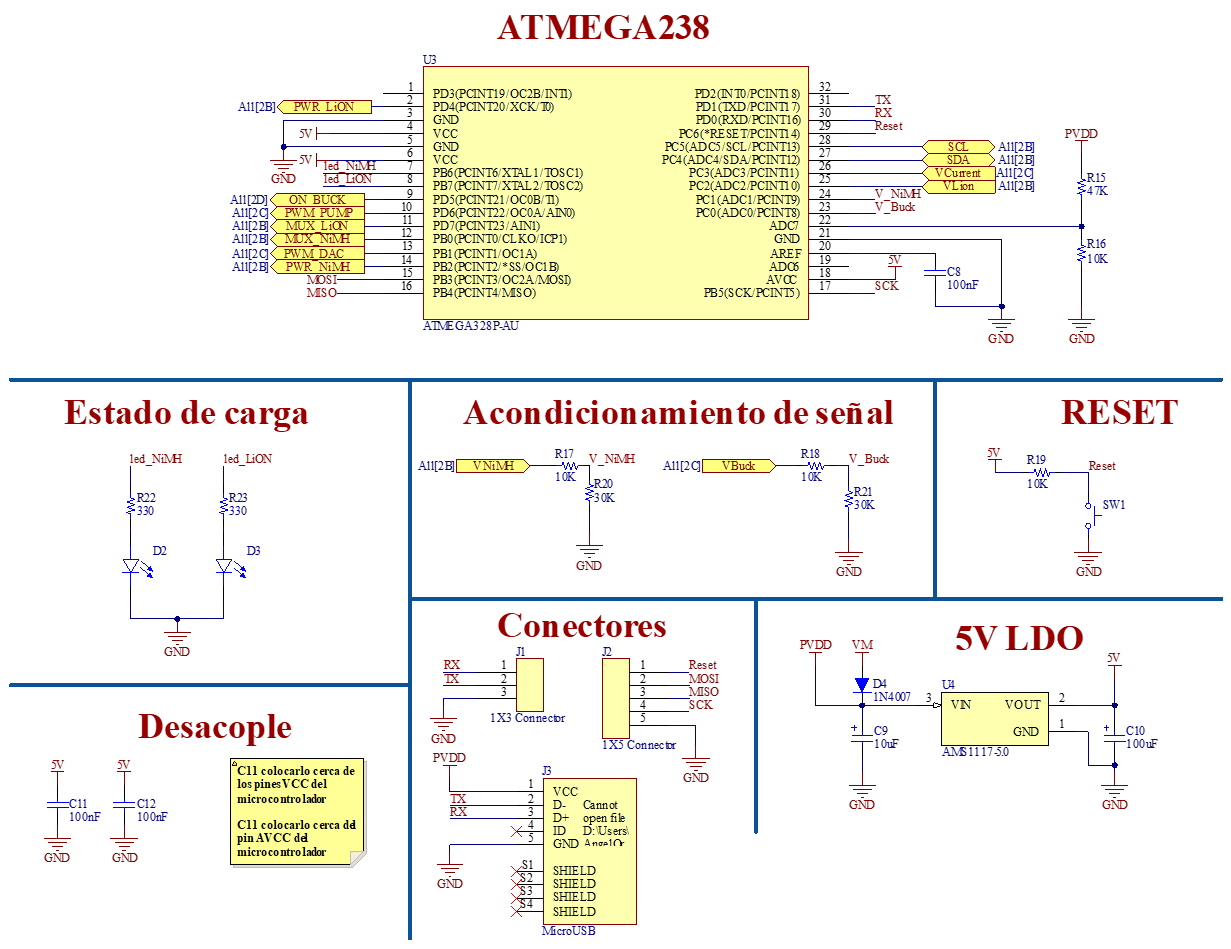
\includegraphics[scale=0.45]{imagenes/controlador_disenio.png}
    \caption{Diagrama esquemático del controlador (S1 en la figura \ref{fig:all})}
    \label{fig:controlador_anexo}
\end{figure}

\begin{figure}[H]
    \centering
    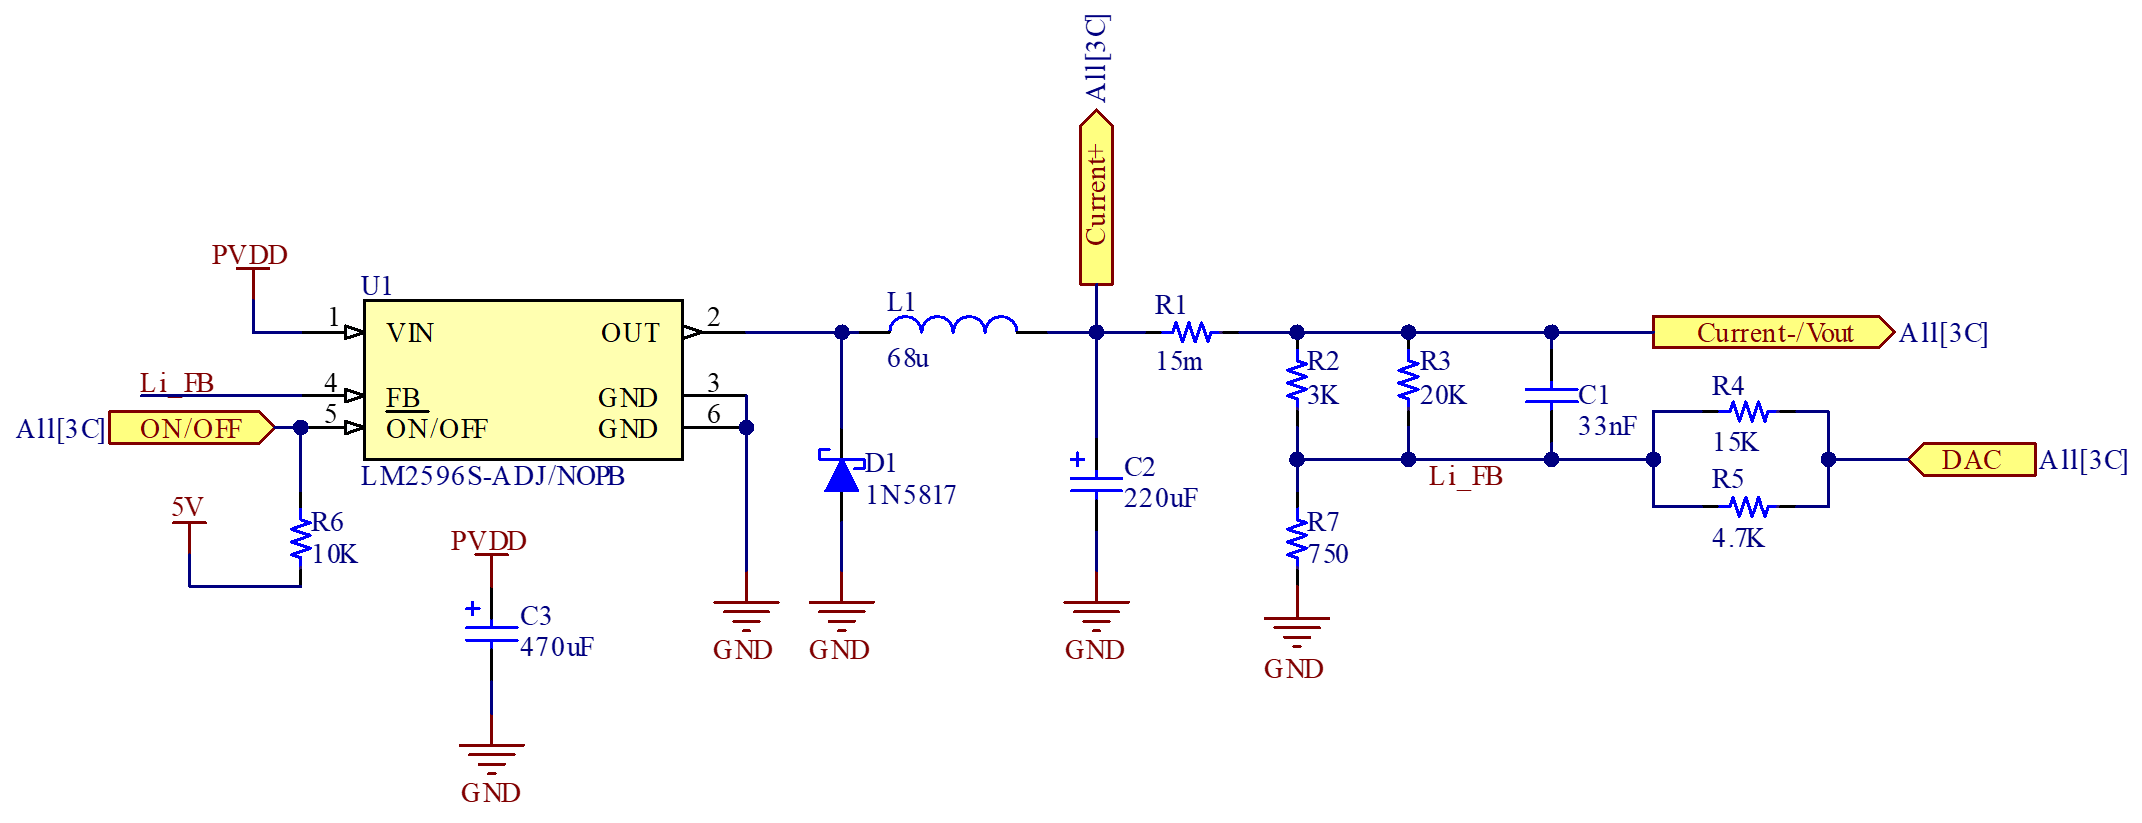
\includegraphics[scale=0.28]{imagenes/charger_anexos.png}
    \caption{Diagrama esquemático del convertidor reductor (S3 en la figura \ref{fig:all})}
    \label{fig:charger_anexo}
\end{figure}

\begin{figure}[H]
    \centering
    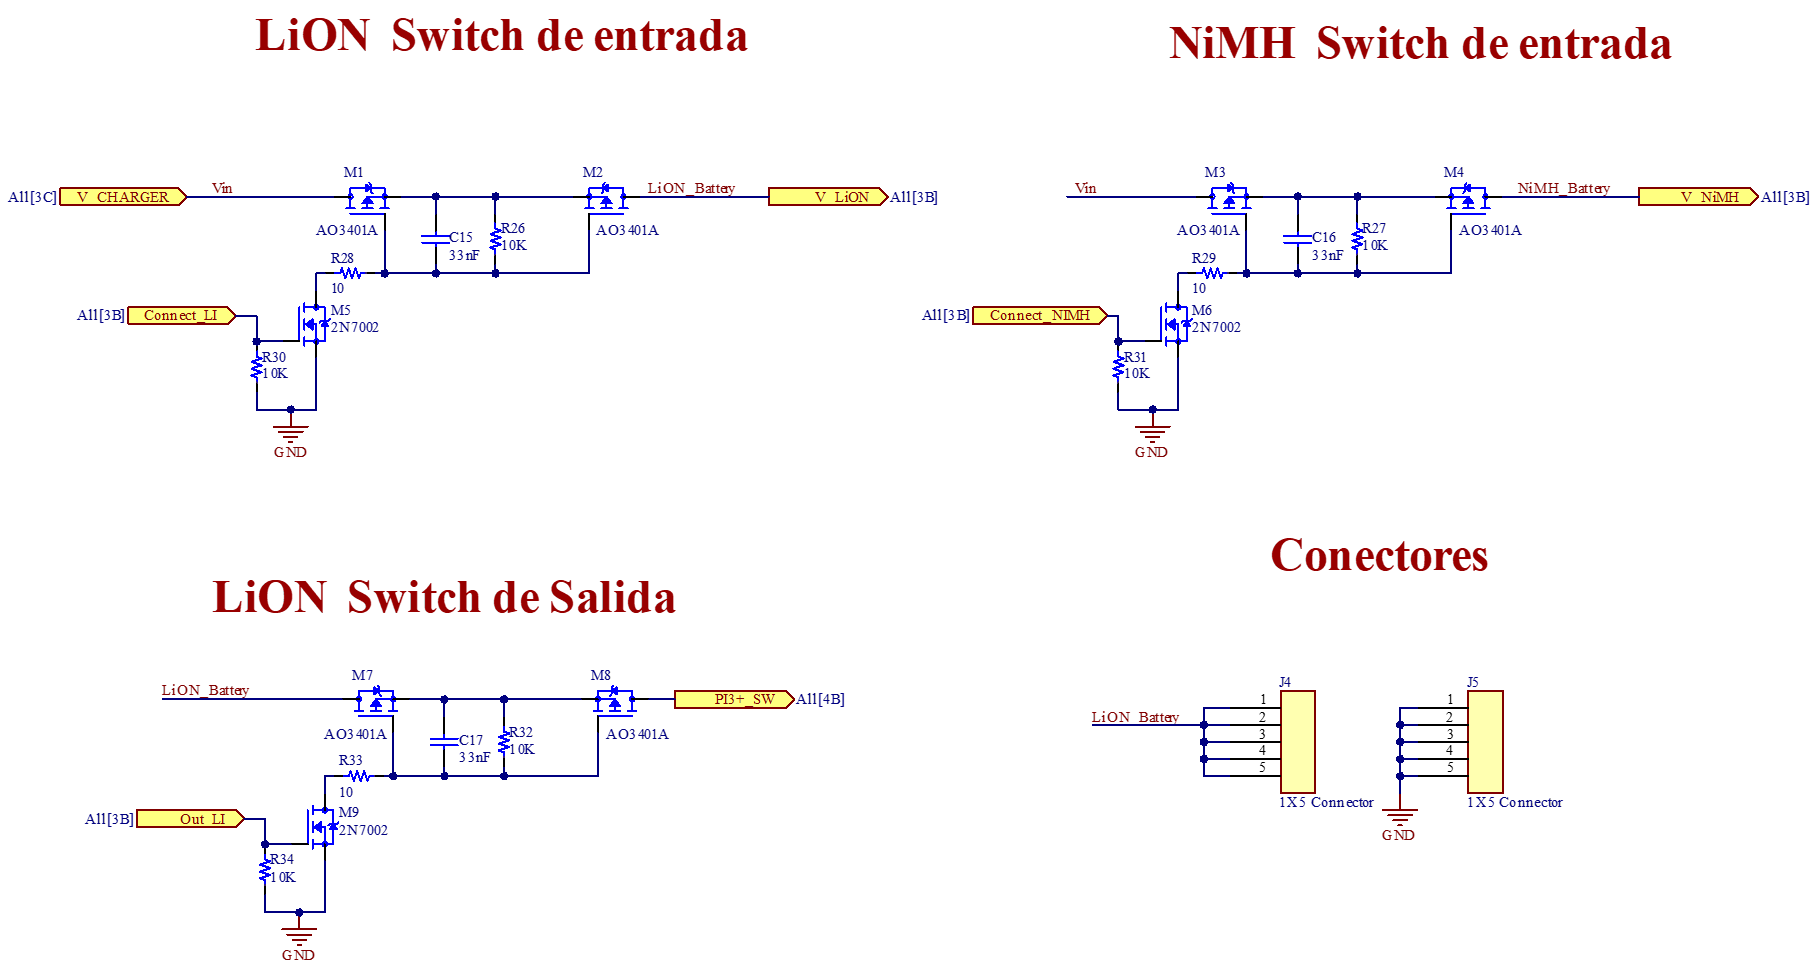
\includegraphics[scale=0.3]{imagenes/mux_anexo.png}
    \caption{Diagrama esquemático del multiplexor de potencia (S6 en la figura \ref{fig:all})}
    \label{fig:charger_anexo_mux}  
\end{figure}

\begin{figure}[H]
    \centering
    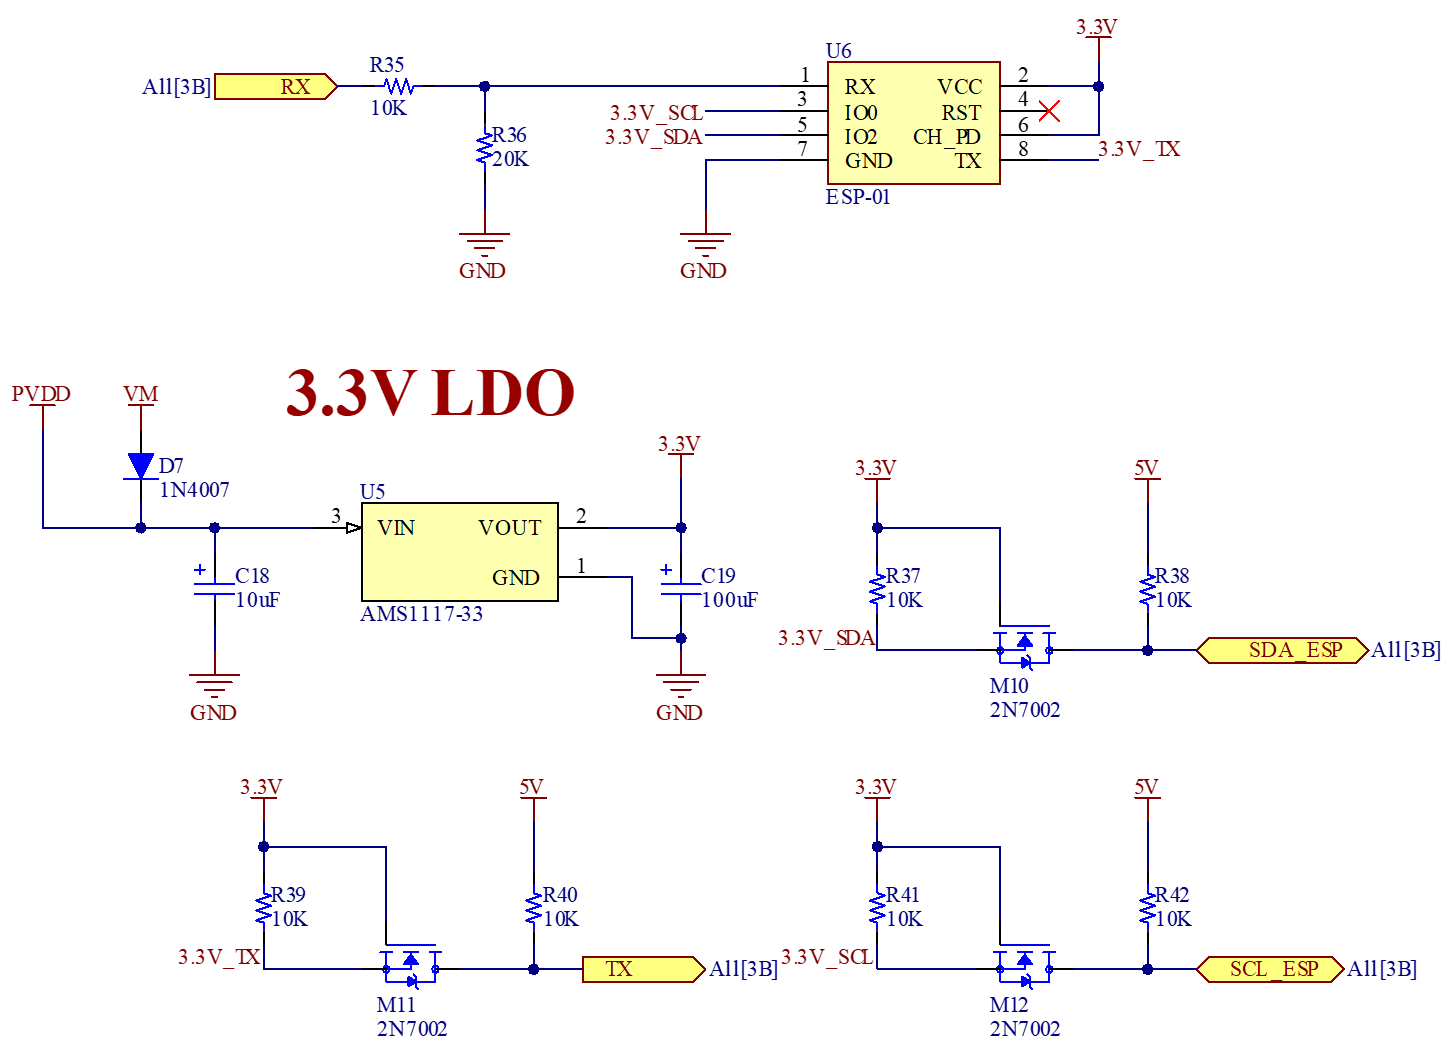
\includegraphics[scale=0.3]{imagenes/esp01.png}
    \caption{Diagrama esquemático del ESP01}
    \label{fig:esp01_anexo}
\end{figure}

\begin{figure}[H]
    \centering
    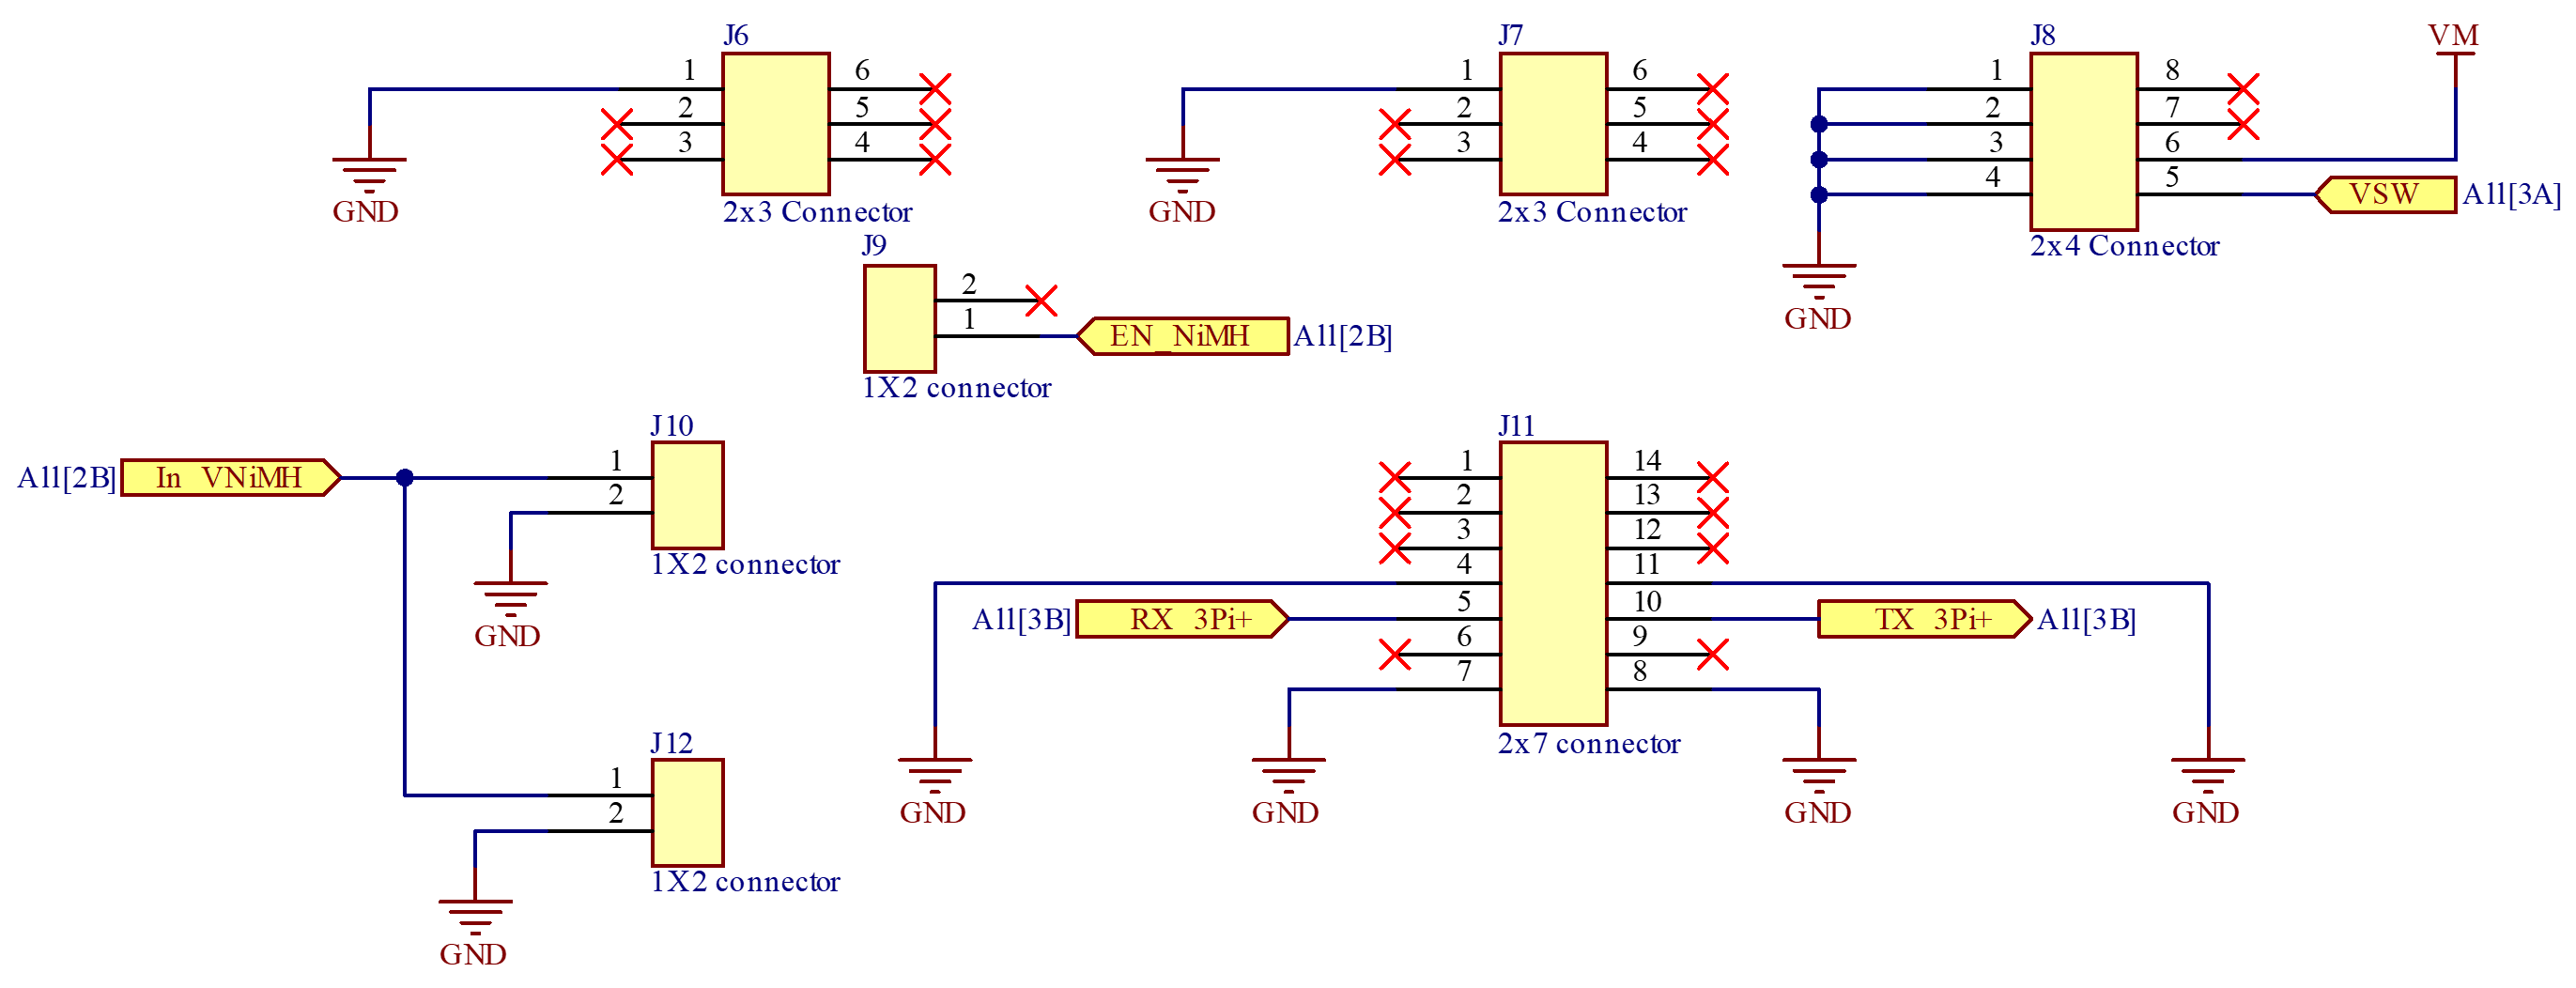
\includegraphics[scale=0.2]{imagenes/3pi+_anexo.png}
    \caption{Diagrama esquemático para los conectores del 3Pi+}
    \label{fig:3pi+_anexo}
\end{figure}

\section{Código fuente empleado en la prueba del DAC}

\label{sec:codigo_dac}

\lstinputlisting[style=atmega328]{../Charge_system_firmware/DAC_test.X/main.c}
\begin{table}[H]
    \caption{Código para prueba de funcionamiento del DAC}
\end{table}

\section{Código fuente empleado en la prueba de funcionamiento de la placa de expansión}
\label{sec:codigo_prueba_expansion}
%\lstinputlisting[style=atmega328]{../Charge_system_firmware/Pololu_on_test.X/main.c}
\begin{table}[H]
    \caption{Código para prueba de funcionamiento de la placa de expansión}
\end{table}
